%%%%%%%%%%%%%%%%%%%%%%%%%%%%%%%%%%%%%%%%%%%%%%%%
% E.Pinault-Bigeard - e.pinault-bigeard@upsti.fr
% http://s2i.pinault-bigeard.com
% CC BY-NC-SA 2.0 FR - http://creativecommons.org/licenses/by-nc-sa/2.0/fr/
%%%%%%%%%%%%%%%%%%%%%%%%%%%%%%%%%%%%%%%%%%%%%%%%
\documentclass[11pt, multicol]{article}
%%%%%%%%%%%%%%%%%%%%%%%%%%%%%%%%%%%%%%%%%%%%%%%%
% Package UPSTI_Document
%%%%%%%%%%%%%%%%%%%%%%%%%%%%%%%%%%%%%%%%%%%%%%%%
%%%%%%%%%%%%%%%%%%%%%%%%%%%%%%%%%%%%%%%%%%%%%%%%
% Package UPSTI_Document
%%%%%%%%%%%%%%%%%%%%%%%%%%%%%%%%%%%%%%%%%%%%%%%%
\usepackage{subcaption}
\usepackage[usenames, svgnames, dvipsnames]{xcolor}
\usepackage{UPSTI_Document}
\usepackage{pgfplots}
\usepackage{import}
\definecolor{darkspringgreen}{rgb}{0.09, 0.45, 0.27}

\newcommandx*{\dessinRepereFigGeo}[5][1=\vx{},2=\vy{},3=\vz{},4=,5=0]
	{
		\draw [->,very thick] (0,0) -- (1,0) ;
		\draw [->,very thick] (0,0) -- (0,1) ;
    \fill[white] (0,0) circle (0.13);
    \draw [->,very thick] (0,0) circle (0.13);
    \ifnumequal{#5}{0} {% z vers nous
      \fill[black] (0,0) circle (0.03);
      \draw [->,thick] (0,0) circle (0.04);
    }{% z vers la feuille
  		\begin{scope} [rotate=45]
  			\draw [-,thick] (0,-0.12) -- (0,0.12) ;
  			\draw [-,thick] (-0.12,0) -- (0.12,0) ;
  		\end{scope}
    }
		\draw [anchor=north west] (1.1,0) node {${#1}$};
		\draw [anchor=south west] (0,1.1) node {${#2}$};
		\draw [anchor=north east] (-0.1,0) node {${#3}$};
		\draw [anchor=north west] (-0.1,-0.1) node {${#4}$};
	}

	\usepackage{array}
	\newcolumntype{L}[1]{>{\raggedright\let\newline\\\arraybackslash\hspace{0pt}}m{#1}}
	\newcolumntype{C}[1]{>{\centering\let\newline\\\arraybackslash\hspace{0pt}}m{#1}}
	\newcolumntype{R}[1]{>{\raggedleft\let\newline\\\arraybackslash\hspace{0pt}}m{#1}}

	\usepackage{pifont}% http://ctan.org/pkg/pifont
\newcommand{\cmark}{\color{green}\ding{51}}%
\newcommand{\xmark}{\color{red}\ding{55}}%
\newcommand{\fmark}{\ding{229}}%
\newcommand{\itemc}{\item[\cmark]}%
\newcommand{\itemx}{\item[\xmark]}%
\newcommand{\itemf}{\item[\fmark]}%

\usepackage{multirow}
%---------------------------------%
% Paramètres du package
%---------------------------------%

% Version du document (pour la compilation)
% 1: Document prof
% 2: Document élève
% 3: Document à publier
\newcommand{\UPSTIidVersionDocument}{2}


% Classe
% 1: PTSI				6: PSI*			11: TSI2		16: Spé
% 2: PT	(par défaut)	7: MPSI			12: ATS
% 3: PT*				8: MP			13: PC
% 4: PCSI				9: MP*			14: PC*
% 5: PSI				10: TSI1		15: Sup
%\newcommand{\UPSTIidClasse}{2}



% Matière
% 1: S2I (par défaut)    2: IPT     3: TIPE
% 6: Vie au lycée
\newcommand{\UPSTIvariante}{5}
\newcommand{\UPSTIidMatiere}{0}
\newcommand{\UPSTIintituleMatiere}{Automatique}
\newcommand{\UPSTIsigleMatiere}{Autom}
% Type de document
% 0: Custom*				7: Fiche Métho de			14: Document Réponses
% 1: Cours (par défaut)		8: Fiche Synthèse    		15: Programme de colle
% 2: TD     				9: Formulaire
% 3: TP						10: Memo
% 4: Colle					11: Dossier Technique
% 5: DS						12: Dossier Ressource
% 6: DM						13: Concours Blanc
% * Si on met la valeur 0, il faut décommenter la ligne suivante:
%\newcommand{\UPSTItypeDocument}{Custom}
\newcommand{\UPSTIidTypeDocument}{1}

% Titre dans l'en-tête


% Titre dans l'en-tête

\newcommand{\UPSTIvariante}{5}

\newcommand{\UPSTItitreEnTete}{Automatisme industriel}
%\newcommand{\UPSTItitreEnTetePages}{}
\newcommand{\UPSTIsousTitreEnTete}{Introduction aux API}


% Titre
%\newcommand{\UPSTItitrePreambule}{Automatisme industriel}
\newcommand{\UPSTItitre}{La programmation d'un Automate Industriel}

% Durée de l'activité (pour DS, DM et TP)
\newcommand{\UPSTIduree}{3h30}

% Note de bas de première page
%\newcommand{\UPSTInoteBasDePremierePage}{Geoffrey Vaquette}
% Numéro (ajoute " n°1" après DS ou DM)
\newcommand{\UPSTInumero}{2}

% Numéro chapitre
%\newcommand{\UPSTInumeroChapitre}{1}

% En-tête customisé
%\newcommand{\UPSTIenTetePrincipalCustom}{UPSTIenTetePrincipalCustom}

% Message sous le titre
%\newcommand{\UPSTImessage}{Message sous le titre}


% Référence au programme
%\newcommand{\UPSTIprogramme}{\EPBComp \EPBCompP{B1-02}, \EPBCompP{B2-49}, \EPBCompS{B2-50}, \EPBCompS{B2-51}, \EPBCompP{C1-07}, \EPBCompP{C1-08}}

% Si l'auteur n'est pas l'auteur par défaut
%\renewcommand{\UPSTIauteur}{WWOOOOOOWW}

% Si le document est réalisé au nom de l'équipe
%\newcommand{\UPSTIdocumentCollegial}{1}

% Source
\newcommand{\UPSTIsource}{G. Vaquette, A. Juton, J. Deprez, J. Maillefert}

% Version du document
\newcommand{\UPSTInumeroVersion}{1.0}

%-----------------------------------------------
\UPSTIcompileVars		% "Compile" les variables
%%%%%%%%%%%%%%%%%%%%%%%%%%%%%%%%%%%%%%%%%%%%%%%%


%%%%%%%%%%%%%%%%%%%%%%%%%%%%%%%%%%%%%%%%%%%%%%%%
% Début du document
%%%%%%%%%%%%%%%%%%%%%%%%%%%%%%%%%%%%%%%%%%%%%%%%
\newcommand{\nomTP}{ascenseurCAN}
\begin{document}
\UPSTIbuildPage
\UPSTIobjectif{\begin{itemize}
	\item Reconnaissance de la partie opérative
	\item Identification des capteurs et des actionneurs
 	\item Identification des éléments de la commande
	\item Prise en main de l’outil de développement
 	\item Mise au point de programmes de test
\end{itemize}}

\tableofcontents


\section{Introduction}
\begin{figure}[ht]
	\centering
	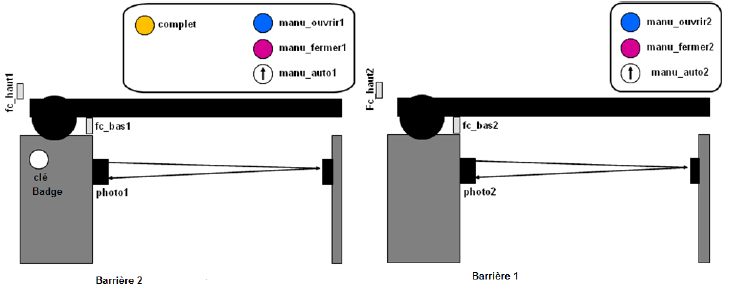
\includegraphics[width=.8\linewidth]{images/schemaSysteme}
	\caption{Partie opérative du système de tri de pièce}
	\label{fig:schemaPartieOperative}
\end{figure}
Ce TP porte sur une maquette de système de stockage temporaire de pièce (Figure~\ref{fig:schemaPartieOperative}). Ce système est piloté par un automate programmable MODICON de la marque SCHNEIDER. On fera, dans un premier temps, un test des capteurs et des actionneurs.
Le développement se fera à l'aide du logiciel \textbf{EcoStruxure} de \textit{Schneider Electric}. Ce TP traite majoritairement d'un comportement séquentiel qui sera implémenté à l'aide de GRAFCET.

\section{Partie opérative}
\subsection{Description}
L’appareil s’intercale entre deux machines de production et a pour fonction d’absorber les
irrégularités de production de la machine amont ou de consommation de pièces de la machine
aval (Figure~\ref{fig:schemaPartieOperative}).
Par exemple, la machine 1  est plus rapide que la machine 2 mais travaille irrégulièrement. Pendant
les arrêts de la machine 1, le stock diminue. Pendant ses phases de production, le stock
augmente. Grâce au stock tampon, la machine 2 travaille en continu à son maximum de
capacité~\ref{fig:application}.

\begin{figure}
	\begin{subfigure}{0.49\textwidth}
	\centering
		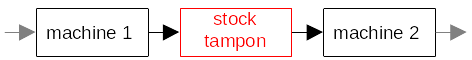
\includegraphics[width=\textwidth]{images/fluxPiece}
		\caption{Signal analogique}
	\end{subfigure}%
	\begin{subfigure}{.49\textwidth}
		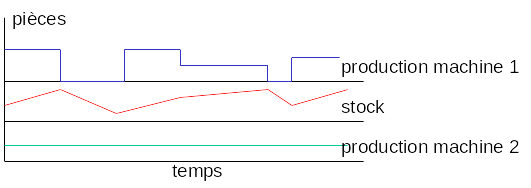
\includegraphics[width=\textwidth]{images/graphPiece}
		\caption{Flux des pièces}
	\end{subfigure}
	\caption{application d'un stockage temporaire de pièces}
	\label{fig:application}
\end{figure}

Les pièces sont acheminées par un convoyeur entraîné par le moteur MC.
En phase de stockage, les pièces sont arrêtées par un bloqueur actionné par le vérin de déplacement horizontal VB et comportant un détecteur de proximité inductif DPI4.
La pièce est saisie par une ventouse EA solidaire du vérin de déplacement vertical VEA.
Le bras manipulateur, entraîné transversalement par le moteur MT et longitudinalement par le
vérin VL permet de stocker la pièce sur une palette à 6 emplacements. Quatre détecteurs de
proximité inductifs DPI0, DPI1, DPI2 et DPI3 alignés le long du guide transversal renseignent sur
la position du bras manipulateur.
En phase de déstockage, la ventouse saisit la pièce à déstocker et la positionne sur le
convoyeur.
Plusieurs modes de fonctionnement sont possibles :
\begin{itemize}
	\item FIFO (First In First Out) qui préserve l’ordre de production des pièces,
	\item  Au plus vite : on pose les pièces dans la case vide la plus proche et on les prend dans la case
	pleine la plus proche.
\end{itemize}

\subsection{A propos du bras manipulateur trois axes}
Le manipulateur 3 axes se déplace selon 3 axes : \textbf{transversal, longitudinal et vertical}.

\paragraph{Mouvement transversal (perpendiculaire au convoyeur) }La transmission mécanique comporte une courroie. Le câblage du moteur autorise la marche
avant et la marche arrière. La position est contrôlée par quatre détecteurs de position, DPIn
correspondant à la position de saisie/dépose sur le convoyeur et aux trois positions de stockage.
Deux contacteurs de fin de course FC1 et FC2 coupent l’alimentation du moteur en butée
mécanique. Pour autoriser un nouveau fonctionnement, le chariot doit être écarté des butées
(mode manuel).
Il y a une commande pour le déplacement avant et une commande pour le déplacement arrière.

\paragraph{Mouvement longitudinal (parallèle au convoyeur)}
Deux positions, avancée ou reculée, course de 50 mm commandée par un vérin pneumatique.
La même commande (active ou inactive) provoque le déplacement dans un sens ou dans l’autre.

\paragraph{Mouvement vertical }Deux positions : haute et basse, la course est commandée par vérin.
Il y a une commande pour la montée et une commande pour la descente.


\subsection{A propos des actionneurs pneumatiques}
Le montage comporte des actionneurs électriques (comme le moteur) et pneumatiques (les vérins).
La commande de ces actionneurs pneumatiques (vérins simple effet) se fait par l’intermédiaire
d’électro distributeurs (vannes pneumatiques commandées électriquement).

Lorsqu'une tension de 24V est appliquée à la bobine des électro distributeurs, elle provoque la commutation des circuits d’air. L'air comprimé augmente alors la pression d'un côté du corps du vérin associé provoquant la sortie (ou retour) de la tige du vérins.
Pour chacun de ces verins, des capteurs permettent de tester leur état « SORTI » (repérés B5, B6, B7, B8, B9 sur la maquette).

\UPSTIattention{Il faut vérifier que le compresseur de la salle de TP a été mis en marche.}

\section{Partie commande (API)}
La partie commande est assurée par un automate \textit{MODICON} du constructeur \textit{Schneider}. Il dispose d'un module d'entrée TOR et d'un module de sortie TOR.

\UPSTIrappel{\begin{itemize}
	\item Les \textbf{capteurs} de la partie opérative sont reliées aux \textbf{entrées} de l'automate.
	\item Les \textbf{actionneurs} de la partie opérative sont reliées aux \textbf{sorties} de l'automate.
\end{itemize}
}
\subsection{Table d'entrée-sortie de l'automate}
Afin de gagner du temps lors du TP, nous fournissons un projet configuré à l'avance. La table des entrées-sorties est incluse à ce projet (Figure~\ref{fig:entreesSorties})
\begin{figure}[h]
	\centering
	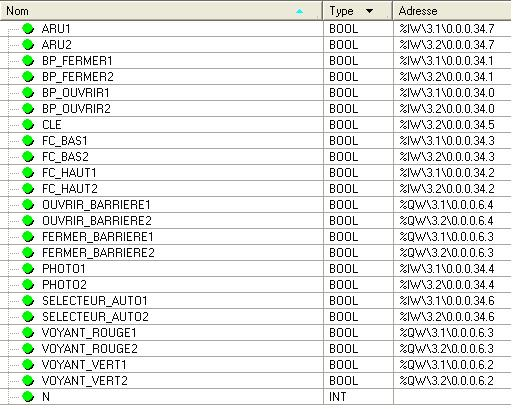
\includegraphics[width=.9\textwidth]{images/listeES}
	\caption{Table des entrées et sorties au sein du projet}
	\label{fig:entreesSorties}
\end{figure}
\pagebreak
\section{Travail demandé}
\subsection{Mise en place informatique}
\begin{UPSTIactivite}[3][Structure du répertoire]
	Dans votre dossier personnel,
	\begin{enumerate}
		\item Créer un dossier intitulé TP03-\nomTP (ou TP04-\nomTP)
		\item Dans ce dossier, créer un dossier \textit{compte-rendu}
		\begin{itemize}
			\item Il contiendra les images, données et le compte-rendu en lui-même
		\end{itemize}
		\item Créer un dossier \textit{projetEcostruxure}
		\item Y copier le contenu du dossier \textit{\nomTP} fourni sur \textit{Commun/Automatisme\_et\_distribution}

	Une fois votre dossier configuré, nous allons compiler et envoyer le projet sur l'automate pour vérifier que la communication entre le PC et l'automate est fonctionnelle.

		\item Ouvrir le projet à l'aide du logiciel \textit{EcoStruxure}
		\item Mettre l'automate sous tension puis compiler et transférer le programme.
		\item Lancer le programme sur l'automate (\textbf{Exécuter})
	\end{enumerate}
\end{UPSTIactivite}

\subsection{Consignes et conseils pour la rédaction du compte-rendu}
Vous rédigerez un compte-rendu détaillé des manipulations effectuées celui du TP 3 servira d'entraînement et comptera avec un coefficient moins important que celui du TP4.

\UPSTIremarque{
Le compte-rendu évalue votre capacité à \textbf{expliquer et synthétiser} votre démarche et les manipulations effectuées.
Les manipulations en elle-même sont observées durant la séance par l'enseignant.}

Vous pourrez donc insérer des captures d'écrans, photos et tout schéma pouvant aider à la compréhension de votre propos.
Un bon compte-rendu est un compte-rendu \textbf{lisible et entièrement compréhensible} par une personne n'ayant pas participé au TP et ayant un niveau de connaissance similaire au vôtre.

\subsection{Prise en main et vérification du fonctionnement du système}
La première chose à vérifier avant d'entreprendre la programmation d'un automate est de vérifier le bon fonctionnement des entrées et sorties de l'automate.
\begin{UPSTIactivite}[][Test des capteurs]
	Avec l'automate sous tension, vérifier \textbf{un à un} le bon fonctionnement de \textbf{tous les capteurs} en vérifiant que la LED correspondante sur le module d'entrées s'allume ainsi que le changement d'état dans la table d'animation du projet.

	Si un capteur ne fonctionne pas ou que son état ne varie pas dans la table d'animation, chercher alors la cause de ce disfonctionnement.
\end{UPSTIactivite}
\UPSTIboiteGenerique{Aide à la rédaction}{\bcplume}{
A titre d'exemple, pour la présentation des tests des capteurs dans votre compte-rendu, vous pouvez expliquer la démarche générale puis insérer une capture d'écran du test d'un des capteurs avec l'explication associée. Il n'est pas alors nécessaire de faire une capture pour chaque capteur.

Précisez également s'il s'agit d'une structure locale ou déportée et décrivez tout disfonctionnement rencontré et comment il a été corrigé.}

\begin{UPSTIactivite}[][Test des actionneurs]
Pour tester les actionneurs, il est nécessaire de commander les sorties de l’automate.

Dans la table d'animation, cliquer sur \textit{Modifications} afin d'activer la commande des sorties.

Vérifier \textbf{un à un} le bon fonctionnement de \textbf{tous les actionneurs} en vérifiant que la LED correspondante sur le module de sortie s'allume et que l'actionneur s'active.
\end{UPSTIactivite}


\subsection{Programmation de l'automate}
\subsubsection{Stockage d'une pièce}
On propose le cahier des charges suivant :
\UPSTIboiteGenerique{Cahier des charges 1 : stockage d'une pièce}{\bcoutil}{
\begin{itemize}
	\item Le stockage ne se fait que si le commutateur 3 positions est en position droite.
	\item La procédure de stockage est engagée par action sur le bouton poussoir Départ Cycle
	\item Le voyant bleu est allumé durant toute l'opération de stockage
	\item La procédure de stockage est la suivante :
	\begin{enumerate}
		\item Sortie du vérin de blocage
		\item Avance du convoyeur jusqu'à détection d'une pièce bloquée
		\item Saisie de la pièce et stockage en position 4
		\item Extinction du voyant et attente d'un nouveau cycle
	\end{enumerate}
\end{itemize}}

\begin{UPSTIactivite}[][Implémentation du Cahier des charges 1]
	\label{act:montee}
	\begin{enumerate}
		\item Dessiner, sur papier ou à l'aide d'un logiciel adapté, le GRAFCET à implémenter
		\item Créer une section dans le projet et implémenter la structure du GRAFCET
		\item Ajouter un commentaire à côté de chage action pour décrire les actions voulues
		\item Implémenter les transitions (penser à créer des sections transitions au besoin, donner des noms \textbf{compréhensibles})
		\item Ajouter et implémenter une section transitions (LADDER ou ST) pour l'activation des actionneurs
	\end{enumerate}
\end{UPSTIactivite}
\UPSTIboiteGenerique{Aide à la rédaction}{\bcplume}{
	A titre d'exemple, dans votre compte-rendu, vous pouvez insérer le GRAFCET ainsi que la section actionneurs. Vous pouvez également expliquer la démarche pour construire un des réseaux du programme LADDER.
}

\subsubsection{Déstockage d'une pièce}
\UPSTIboiteGenerique{Cahier des charges 2 : Déstockage}{\bcoutil}{
	\begin{itemize}
		\item Le déstockage ne se fait que si le commutateur 3 positions est en position \textbf{gauche}.
		\item La procédure de déstockage est engagée par action sur le bouton poussoir Départ Cycle
		\item Le voyant bleu est allumé durant toute l'opération de stockage
		\item La procédure de stockage est la suivante :
		\begin{enumerate}
			\item Saisie de la pièce en position 4
			\item Dépose sur le convoyeur
			\item Avance du convoyeur pendant 3 secondes
			\item Extinction du voyant et attente d'un nouveau cycle
		\end{enumerate}
	\end{itemize}}

\begin{UPSTIactivite}[][Implémentation du Cahier des charges 2]
\begin{itemize}
	\item En suivant la même démarche que pour l'activité~\ref{act:montee}, implémenter le cahier des charges 2.
	Modifier la section actionneurs.
	\item Ajouter les conditions suivantes :
	\begin{itemize}
		\item Le stockage est autorisé s’il n’y a pas de pièce sur l’emplacement 4
		\item Le déstockage est autorisé s’il y a une pièce sur l’emplacement 4
	\end{itemize}
\end{itemize}
\end{UPSTIactivite}

\begin{UPSTIactivite}[2][Pour aller plus loin : Stockage de plusieurs pièces]
	Implémenter le stockage et le déstockage de plusieurs pièces (si l'emplacement 4 est occupé, le stockage se fait sur l'emplacement 1, puis 2, etc.)
\end{UPSTIactivite}

\end{document}
